\section{Class Loading}

\subsection{Java Class Loader}

\subsubsection{About the Java Class Loader}

\textbf{Class Loader}
\\
Defined by the abstract class \textbf{ClassLoader} and its subcalsses.\\
- e.g., SecureClassLoader, URLClassLoader,...

A class loader is an object responsible of loading the classes.

Given the name of a class,

\begin{itemize}
	\item it locates the class according to the class loader rules or
	\item it generates the data (array of bytes) that constitutes a definition for the class
\end{itemize}

and makes it available to the running application.

Class loaders define namespaces.

\begin{itemize}
	\item Every Class object contains a \textbf{Class\#getClassLoader()} reference to the \textbf{ClassLoader} that defined it.
	\item <Class A loaded by CL1> = <Class A loaded by CL2> <> CL1 = CL2
\end{itemize}

\subsubsection{Class Loaders and Name Spaces}

\begin{center}
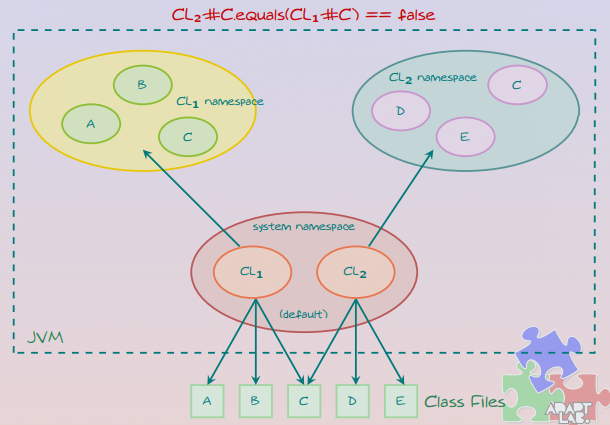
\includegraphics[scale=0.7]{13-class-loader-namespace}
\end{center}

\subsubsection{Effect of the Namespaces: A Broken Singleton}

\begin{lstlisting}[language=Java]
public class Singleton {
	static private boolean runOnce = false;
	public Singleton() {
		if (runOnce)
			throw new IllegalStateException("[ERROR] re-instantiation of «Singleton»!!!");
		runOnce = true;
	}
}
\end{lstlisting}

\begin{lstlisting}[language=Java]
public class SingletonViolationTest {
	public static void main(String[] 	args) throws Exception {
	SimpleClassLoader CL1 = new 	SimpleClassLoader("testclasses");
	Class<?> c1 = 	CL1.loadClass("Singleton");
	println("Loaded class «Singleton» via the «CL1» class loader");
	Field flag = 	c1.getDeclaredField("runOnce"); 	flag.setAccessible(true);
	println("Let’s instatiate 	«Singleton@CL1»\n### runOnce :- 	"+flag.get(null));
	Object x = c1.getDeclaredConstructor().newInstance();
println("### runOnce :- "+flag.get(null));
	try {
		println("Let’s re-instantiate «Singleton@CL1»\n### runOnce :- "+flag.get(null));
		Object y = c1.getDeclaredConstructor().newInstance() ;
		throw new RuntimeException("Test Fails!!!");
	} catch (Exception e) { println(e.getCause().getMessage()); }
	SimpleClassLoader CL2 = new SimpleClassLoader("testclasses");
	println("Loaded class «Singleton» via the «CL2» class loader");
	Class<?> c2 = CL2.loadClass("Singleton");
	Field flag2 = c2.getDeclaredField("runOnce"); 	flag2.setAccessible(true);
	println("Let’s instatiate «Singleton@CL2»\n### runOnce :- "+flag2.get(null));
Object z = c2.getDeclaredConstructor().newInstance();
println("### runOnce :- "+flag.get(null));
	}
}
\end{lstlisting}

\begin{lstlisting}[language=Java]
[11:34]cazzola@hymir:~/tsp>java SingletonViolationTest
Loaded class «Singleton» via the «CL1» class loader
Let’s instatiate «Singleton@CL1»
### runOnce :- false
### runOnce :- true
Let’s re-instantiate «Singleton@CL1»
### runOnce :- true
[ERROR] re-instantiation of «Singleton»!!!
Loaded class «Singleton» via the «CL2» class loader
Let’s instatiate «Singleton@CL2»
### runOnce :- false
### runOnce :- true
\end{lstlisting}

\subsubsection{Why Subclass the Class Loader?}

\textbf{Applications implement subclasses of ClassLoader in order}
\begin{itemize}
	\item to extend the manner in which the Java virtual machine dynamically loads classes;
	\item to obtain different protected name spaces; ands
	\item to transform bytecode!
\end{itemize}

\textbf{Some applications related to the class loaders are:}
\begin{itemize}
	\item Securty
	- examine classes for a proper digital signature
	- disallow the loading of particular packages (for example, java.io)
	\item Encrypting
	-  decrypt classes on the fly, so that your class files on disk are not readable by someone with a decompiler
	\item Archiving
	- distribute your code in a special format or with special compression
	\item Testing
	- keep context for test cases sandboxed/separated by using different loaders
\end{itemize}

\subsubsection{Another Reason to Create Your Own Class Loader}

\textbf{Problem}

Write a method that outputs the inheritance hierarchy of an
application.

\textbf{Subproblem}

How do you discover what classes belong to your application?

\textbf{Solution}

Impossible - The subproblem is extrinsic to Java meta-object
protocol.

\textbf{So what can we do?}

\begin{center}
\textbf{Create our own class loader}
\end{center}

The class loader object knows what classes have been loaded.

\subsubsection{java.lang.ClassLoader}

\begin{lstlisting}[language=Java]
public class ClassLoader {
	protected ClassLoader() { ... }
	protected ClassLoader(ClassLoader parent) { ... }
	public final ClassLoader getParent() { ... }
	public static ClassLoader getSystemClassLoader()
			throws SecurityException, IllegalStateException { ... }
	public static ClassLoader getPlatformClassLoader() throws 		SecurityException { ... }
	protected Class<?> findClass(String name) throws 	ClassNotFoundException { ... }
	protected Class<?> findClass(String moduleName, String name)
throws ClassNotFoundException { ... }
	protected Class<?> findLoadedClass(String name) { ... }
	protected Class<?> findSystemClass(String name) throws 	ClassNotFoundException { ... }
	public Class<?> loadClass(String name) throws ClassNotFoundException { ... }
	protected final void resolveClass(Class<?> c) throws 	NullPointerException { ... }
	protected Class<?> defineClass (String name, byte[] b, int off, int len)
			throws ClassFormatError { ... }
...
}
\end{lstlisting}

\subsubsection{Class Loading: How It Works}

\begin{center}
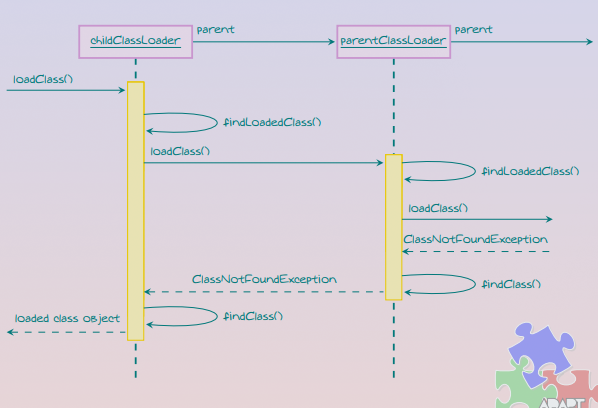
\includegraphics[scale=0.7]{13-java-class-loader}
\end{center}

\textbf{loadClass() is where the loading process start}
\begin{itemize}
	\item it calls findLoadedClass() to check if the class is already loaded;
	\item– if yes it returns the found class otherwise it delegates the task to its parent; Delegation Model.
	\item if everything fails, it invokes the findClass() to find the class, read the bytecode and create the class object (defineClass())
\end{itemize}

\textbf{Something like (Pseudo-Java):}
\begin{lstlisting}[language=Java]
public Class loadClass(String name) throws ClassNotFoundException {
	Class c = findLoadedClass(name);
	if (c != null) return c;
	try {
		return parent.loadClass(name);
	} catch (ClassNotFoundException e) {
		return findClass(name);
	}
}
\end{lstlisting}

\textbf{How to subclass the class ClassLoader:}

\begin{itemize}
	\item create a default constructor and one linking to the parent;
	\item override findClass();
	\item absolutely do not override loadClass() because its original implementation supports the delegation model.
\end{itemize}





The homonym design pattern defines a proxy as an:

\begin{itemize}
	\item object providing a surrogate/placeholder for another object
	\item to control and manipulate the accesses to it
\end{itemize}

Few examples

\begin{itemize}
	\item local representation of remote objects;
	\item delay of expensive operations;
	\item access protection for secure objects.
\end{itemize}

\subsubsection{What Is a Dyniamic Proxy?}

A dynamic proxy class is a class implementing a \textbf{list of interfaces} such that the invocation of a method beloging to one of these interfaces on one of its instances is \textbf{seamleassly dispatched} to another object implementing such interface and bound to the dynamic proxy object.

A dynamic proxy class can be used to create a type-safe proxy object for a set of objects determined by the implemented interfaces \textbf{without} both \textbf{explicit coding} and \textbf{static pre generation} of the proxy class as happens with several compile-time tools.

Dynamic proxy classes are useful to applications or libraries that need to provide type-safe reflective dispatch of invocations on objects whose interface is available

java.lang.reflect.InvocationHandler

\subsubsection{java.lang.reflect.InvocationHandler}

Each proxy instance has an associated invocation handler.

When a method is invoked on a proxy instance

\begin{itemize}
	\item the method invocation is dispatched to the invoke() method of its invocation handler
\end{itemize}

\begin{center}
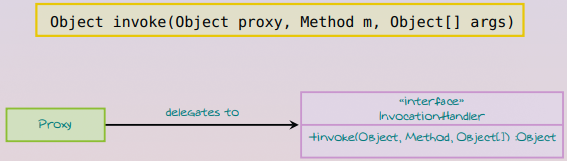
\includegraphics[scale=0.7]{10-invocation-handler}
\end{center}

\subsubsection{java.lang.reflect.Proxy}

Proxy

\begin{itemize}
	\item  provides static methods for creating dynamic proxy classes and instances, and
	\item  it also is the superclass of all dynamic proxy classes created by these methods
\end{itemize}

\begin{lstlisting}[language=Java]
public final class Proxy extends Object implements Serializable {
	protected InvocationHandler h;
	protected Proxy(InvocationHandler h) { ... }
	public static InvocationHandler getInvocationHandler(Object proxy) { ... }
	public static Class<?> getProxyClass(ClassLoader l, Class<?>... interfaces) { ... }
	public static boolean isProxyClass(Class<?> cl) { ... }
	public static Object newProxyInstance(ClassLoader loader, Class<?>[] interfaces, InvocationHandler h ) { ... }
}
\end{lstlisting}

Basically, Proxy enables the meta-object approach in Java

\subsubsection{How Java Creates a Proxy}

\begin{center}
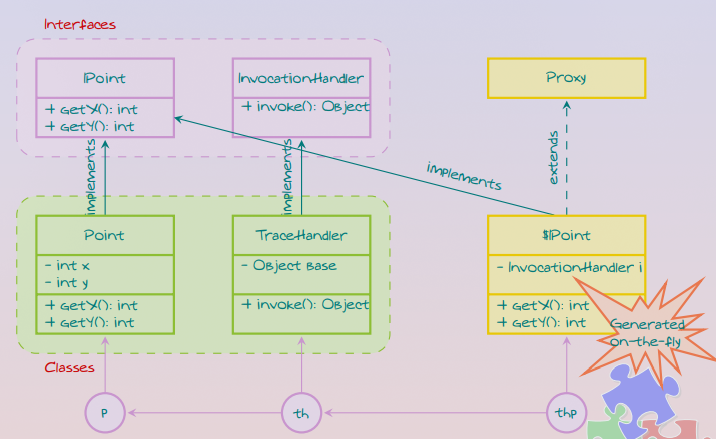
\includegraphics[scale=0.4]{11-create-a-proxy}
\end{center}

\subsubsection{Example: To Trace the Method Calls}

\begin{lstlisting}[language=Java]
import java.lang.reflect.*;
public class TraceHandler implements InvocationHandler {
	private Object baseObject;
	public TraceHandler(Object base) { baseObject = base; }
	public Object invoke(Object proxy, Method m, Object[] args) {
	try {
		System.out.println("before " + m.getName());
		Object result = m.invoke(baseObject, args);
		System.out.println("after " + m.getName());
		return result;
	} catch (Exception e) {
		e.printStackTrace(); 
		return null;
	}
}
public String toString() { return "th :- "+this.baseObject; }
}
\end{lstlisting}

\begin{lstlisting}[language=Java]
jshell> IPoint p1 = new Point(10,20);
p1 ==> p :- (10, 20)
jshell> IPoint th_p1 = (IPoint) Proxy.newProxyInstance(
p1.getClass().getClassLoader(), p1.getClass().getInterfaces(), new TraceHandler(p1));
before toString
after toString
th_p1 ==> p :- (10, 20)
jshell> p1.getX(); /* standard call */
$10 ==> 10
jshell> th_p1.getX(); /* traced call */
before getX
after getX
$11 ==> 10
\end{lstlisting}

\subsubsection{Example: Invariant Checking and Proxy Chaining}

\begin{lstlisting}[language=Java]
import java.lang.reflect.*;

public class InvariantHandler implements InvocationHandler {
	private Object target;
	private Method invariant;
	public InvariantHandler(Object target) {
		this.target = target;
		try {
			invariant = target.getClass().getMethod("invariant", new Class<?>[]{});
			if (!invariant.getReturnType().equals(boolean.class)) invariant = null;
		} 
		catch (NoSuchMethodException ex) { 
			invariant = null; }
		}
		
public Object invoke(Object proxy, Method method, Object[] args) throws Throwable {
	this.invokeInvariant(method);
	Object retvalue = method.invoke(this.target, args);
	this.invokeInvariant(method);
	return retvalue;
}

private void invokeInvariant(Method method) {
	if ((this.invariant == null) || (method.equals(this.invariant))) return;
	try {
		Boolean passed = (Boolean) invariant.invoke(target, new Object[]{});
		if (!passed.booleanValue()) throw new RuntimeException();
	} catch (Exception e) {
		System.out.println("Failed invariant check!!!"); 
	}
}
public String toString() {return "ih :- "+this.target; }
}
\end{lstlisting}

\subsubsection{Example: Invariant Checking and Proxy Chaining (Cont'd)}

\begin{lstlisting}[language=Java]
jshell> InvariantHandler ih = new InvariantHandler(new Point(0, 7));
ih ==> ih :- p :- (0, 7)
jshell> IPoint invariantCheckedPoint =
(IPoint)Proxy.newProxyInstance(
Point.class.getClassLoader(),
new Class[]{ IPoint.class }, ih);
invariantCheckedPoint ==> p :- (0, 7)
jshell> TraceHandler th = new TraceHandler(invariantCheckedPoint);
th ==> th :- p :- (0, 7)
jshell> IPoint tracedInvariantCheckedPoint =
(IPoint)Proxy.newProxyInstance(
Point.class.getClassLoader(),
new Class[] { IPoint.class }, th);
before toString
after toString
tracedInvariantCheckedPoint ==> p :- (0, 7)
jshell> tracedInvariantCheckedPoint.setX(25)
before setX
after setX
jshell> tracedInvariantCheckedPoint.setY(-7)
before setY
Failed invariant check!!!
after setY
\end{lstlisting}

\subsubsection{Example: Invariant Checking and Proxy Chaining (Cont'd)}

\begin{center}
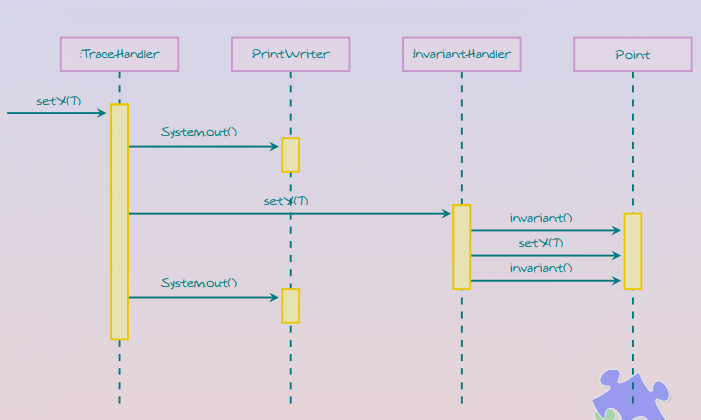
\includegraphics[scale=0.4]{12-proxy-chaining}
\end{center}


 
